\begin{figure}[t]
\centering
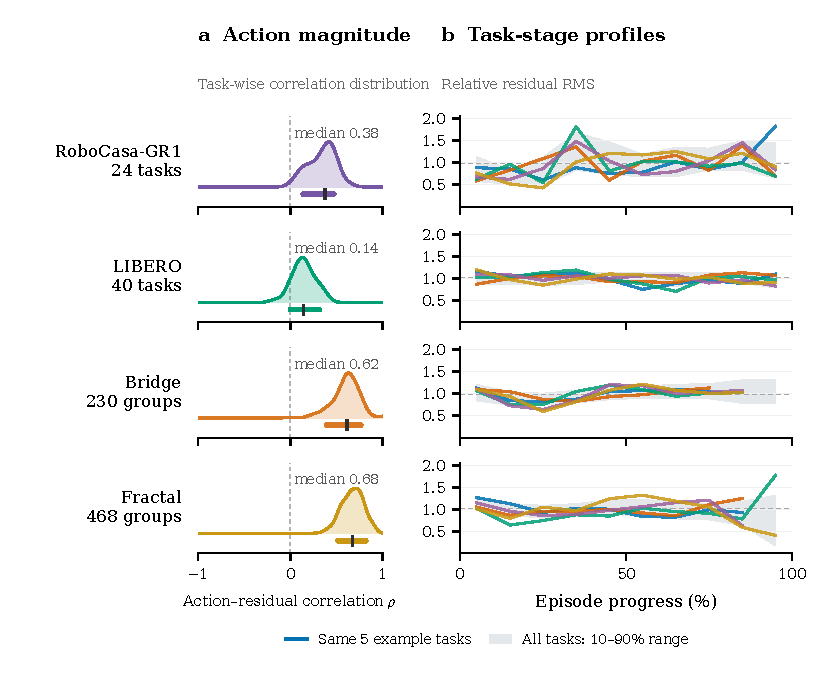
\includegraphics[width=\linewidth]{analysis/diagnostics/crossdataset_residual/all_datasets_progress_clean.pdf}
\caption{\textbf{Action magnitude and stage-dependent regression residuals across datasets.}
(a) Distributions of task-wise Spearman correlations between action RMS and general-MSE residual RMS. Curves are boundary-reflected kernel density estimates; bars indicate the 10th--90th percentiles and ticks indicate medians.
(b) Residual RMS across ten episode-progress bins, divided by each task's root-mean-square bin scale. Five tasks per dataset are sampled with a fixed seed, unchanged from the full-line visualization. Shading shows pointwise 10th--90th percentiles across all qualifying tasks, not confidence intervals; no trajectory smoothing is applied.
Bridge and Fractal include nonempty instruction groups with at least 12 sampled demonstrations. These diagnostics use training-demonstration residuals.}
\label{fig:crossdataset-residual-clean}
\end{figure}
